\chapter{Systematic Uncertainties}
\label{cha:systematics}

Before unveiling the final distribution(s), the various systematic uncertainties have to be taken into consideration. These types of uncertainties describe an additional uncertainty or a possible bias that the methods of the analysis themselves introduce to a measurement or a prediction. To account for them, the parameters of the procedures are usually varied in a way that both over- and underestimations are covered. The relevant uncertainties can be split into two categories. On the one hand there are those that affect the analysis on a global scale, while on the other hand some only concern specific types of objects. Unless stated otherwise, all of the uncertainties are determined using the smuon mass distribution at the final stage of the analysis.

For the signal samples, the systematic uncertainties are estimated from the impact of each individual procedure on the three shown points in the RPV supersymmetry phase space. In most cases, the points with lower values of the universal mass parameters are experiencing the largest relative influence. 

The systematic uncertainty of the data-driven background prediction is evaluated separately. Therefore the global and object uncertainties are only given for Monte Carlo samples which are \textit{not} replaced by the estimate.

\section{Object Uncertainties}
\label{sec:objsys}

\subsection{Jet Energy Resolution}
\label{sec:jersys}

The procedure discussed in section~\ref{sec:jer} describes the adjustment of the jet energy resolution already. It remains the same for estimating its systematic uncertainty. As for the variation of its parameters, the core resolution factors (Tab.~\ref{tab:jerfactors}) are scaled according to their uncertainties. Both the statistical and systematic upper and lower bound are added quadratically and applied to the mean value. While this applies to both cases of matched and no matched gen-jets, the latter can only worsen the resolution. As a result, a core resolution factor is not expected to be less or equal to 1. With the width of the Gaussian distribution used for smearing given by $\sigma = \mathbf{\sqrt{c^2-1}} \cdot \sigma_{\text{MC}}$, values below that threshold have to be adjusted. This is only the case for the lower bound of the $0 < |\eta| < 0.5$ range. Here instead of $0.990$, $1.001$ is used. 

While the statistical error of the energy resolution in the Monte Carlo samples $\sigma_{\text{MC}}$ is negligible, the fitting procedure is subject to systematic uncertainties such as the range it considers, as well. To account for that, the value of $\sigma_{\text{MC}}$ has been varied separately from the core resolution scaling factors by $\pm 5\,\pct$. The effect has been found to be below $0.1\,\pct$.

For the background Monte Carlo samples, the overall effect for an upward deviation then amounts to $-0.1\,\pct$ while for the downward one it is $+0.6\,\pct$. For the signal prediction, it varies in between $1.2\,\pct$ and $3.4\,\pct$.


\subsection{Jet Energy Scale}
\label{sec:jes}

For the jet energy scale (\textbf{JES}), there are a variety of factors which influence the measurement. A collection of all relevant values is being provided by the JetMET working group on their dedicated website~\cite{jes}. It encompasses the following effects: Absolute scale uncertainty, high transverse momentum extrapolation, single pion influence, jet flavour extrapolation, time dependencies, pileup as well as a statistical uncertainty, resolution dependency and central fit dependency which are given relative to the $p_{\text{T}}$ of jets. The quadrature of all contributions yields the total uncertainty. From the recommended set of uncertainty sources, \verb+Summer13_V2_DATA_AK5PFchs+ is used in this analysis. 

Similarly to the jet energy resolution, the effect of scaling the jet energy has also been propagated to $E_{\text{T}}^{\text{miss}}$. Shifting the energies of all jets up and down affects the number of events by $+3.6\,\pct$ and $-2.9\,\pct$, respectively. The signal is affected by up to $7.8\,\pct$.


\subsection{Muon Momentum Resolution \& Scale}
\label{sec:mers}

The systematic uncertainties for the muon momentum resolution and scale have been determined by the Muon POG~\cite{muonid2}. For muons with less than $200\,\text{GeV}$ transverse momentum, the general recommendations are a $0.2\,\pct$ uncertainty on the value of the scale and $0.6\,\pct$ on the resolution. Should the particle exceed that $p_{\text{T}}$ threshold, the uncertainty on the scale increases with $5\,\pct \cdot p_{\text{T}}/\text{TeV}$. As studies with cosmic are used for measuring the uncertainty on the resolution, the signal topology is not described accurately. By assuming a continuous $30\,\pct$ relative uncertainty on the resolution, based off the $0.6\,\pct$ for $p_{\text{T}} < 200\,\text{GeV}$, the remainder of the spectrum~\cite{muonptscale} is estimated over three regions. The values used for smearing are $1.1\,\pct$ for $p_{\text{T}} < 350\,\text{GeV}$, $1.65\,\pct$ for $p_{\text{T}} < 500\,\text{GeV}$ and $3.1\,\pct$ beyond that transverse momentum.

Applying the resolution uncertainties is performed similarly to the smearing of the jet energy scale in case of no matched gen-jets. Random numbers following a Gaussian distribution are generated, with the width being given by the listed percentages. The energies of muons on the other hand, are shifted by the respective amount to estimate the impact of the muon momentum scale. Once again, all effects are being propagated to $E_{\text{T}}^{\text{miss}}$.

For the resolution, the result is a $0.2\,\pct$ difference. Varying the scale yields a $+0.2\,\pct$ and $-0.2\,\pct$ difference for the up- and downward direction, respectively. In case of the signal Monte Carlo, the impact for the resolution goes up to $3.0\,\pct$, while it only goes up to $1.0\,\pct$ for the scale.


\subsection{Muon  ID Efficiency}
\label{sec:muonidsys}

Possible discrepancies between data and simulation when applying the tight muon ID have been researched by the Muon POG. The scale factors have been determined on the 2012 re-reconstructed datasets, which are also used in this analysis. They are below $1\,\pct$ throughout the entire $\eta$-range for muons beyond the $p_{\text{T}} > 20\,\text{GeV}$ threshold~\cite{muonideff}. 

To compensate for not scaling the number of events accordingly, a conservative $1\,\pct$ systematic uncertainty for both the background as well as the signal is assumed here.


\subsection{B-Tagging}
\label{sec:btagsys}

To estimate the systematic uncertainty for the $b$-tagging algorithm described in section~\ref{sec:bjets}, its scale factor functions are shifted up and down. These variations are taken from the same text files linked on the corresponding website~\cite{btagtwiki}.

Shifting the efficiency maps only yields minor corrections. As (pseudo-)randomly generated numbers are used to determine when to up- or downgrade a jet, the statistical uncertainty overshadows the systematic one. Especially for points in the $p_{\text{T}}$-$\eta$-parameter space with a very low number of entries, the statistical variance is large. For these reasons, their small impact is neglected.

The effect on the smuon mass distribution is $-0.6\,\pct$ for the upward variation and $+0.2\,\pct$ for the downward one. Its impact on the signal lies in between $0.2\,\pct$ and $1.4\,\pct$. 



\section{Global Uncertainties}
\label{sec:glblsys}

\subsection{Luminosity}
\label{sec:lumisys}

The offline estimate of the luminosity uses the information provided by the pixel detector. Since the high granularity allows for a very accurate measurement of the pixel clusters on which the estimate is based on, the uncertainty is comparatively low. For the 2012 datasets, it is $2.6\,\pct$~\cite{lumisys}. It applies directly to all backgrounds as they scale linearly with it.


\subsection{Cross sections}
\label{sec:xssys}

When determining the cross section of a process, there are two main contributions to the uncertainty of the scale: The factorization and renormalization scale. By convention, these are varied up and down by a factor of two to estimate their individual uncertainties. They are also assumed to be fully correlated.

The scale uncertainties have been provided alongside their cross sections for a sizeable portion of Monte Carlo samples. For the remainder, a conservative $50\,\pct$ and $5\,\pct$ uncertainty are assumed for leading order and higher order cross sections, respectively.

For all signal Monte Carlo samples, the estimates given by the authors of the cross section calculation tool are used. They amount to $5\,\pct$ from the scale uncertainty and an additional $7\,\pct$ from supersymmetric QCD processes~\cite{susyxstool}.


\subsection{Parton Distribution Functions}
\label{sec:pdfsys}

With the LHC being a \textit{hadron} collider, the particles it accelerates have a substructure. The constituents of a proton collide and only a fraction $x_i \: (i = 1,2)$ of the center-of-mass energy $s$ enters the interaction: $\hat{s} = x_1 x_2 \cdot s$. A significant part of an accurate Monte Carlo simulation is a precise description of these ``partons'', as the constituents are called. To obtain the cross section $\sigma$ for a selected process, one has to sum over all possible partons and integrate over the energy fractions they can carry.

\begin{equation}
  \label{eq:pdfxs}
  \sigma = \sum_{ij} \int_0^1 \int_0^1 \text{d}x_1 \text{d}x_2 f(x_1, Q^2) f(x_2 ,Q^2) \hat{\sigma}_{ij}(\hat{s})
\end{equation}

Here $\hat{\sigma}_{ij}$ denotes the cross section for the interaction of the partons $i$ and $j$ at their center-of-mass energy $\hat{s}$. The parton density functions (\textbf{PDFs}) $f(x_i, Q^2)$ describe the probability to find a particular parton with a certain energy fraction $x_i$. This likelihood also depends on the energy scale $Q^2$, at which the function is evaluated. PDFs have to be determined experimentally, as it is not possible to predict them from theory alone. Measurements from different experiments and different methods to estimate the evolution of the functions have been used to generate multiple sets of parton distribution functions for the LHC and other experiments. The following three are considered in this analysis to calculate the systematic uncertainty introduced by choosing a particular one~\cite{pdfforlhc}. Both \textsc{MSTW2008}~\cite{mstw2008,mstw2008as} and \textsc{CT10}~\cite{ct10} are optimizing their PDF fit by minimizing a log-likelihood function, while \textsc{NNPDF 2.3}~\cite{nnpdf23,nnpdf23as} uses a template method to determine the closest match to the measurement. Exemplary distributions of \textsc{MSTW2008} for two energy scales are given in figure~\ref{fig:mstw2008pdf}.

\begin{figure}[htb!]
  \centering
  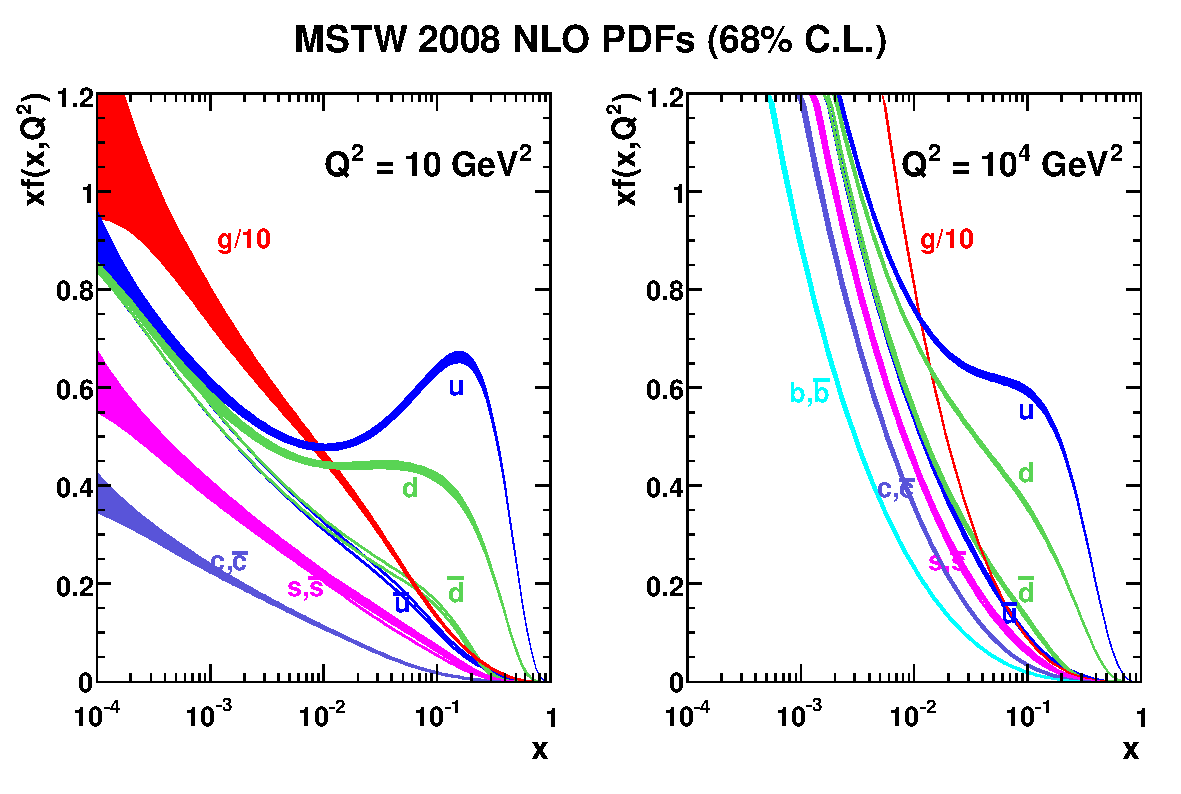
\includegraphics[width=0.7\textwidth]{plots/mstw2008pdf.pdf}
  \caption{Parton distribution functions of the MSTW2008 set at two different energy scales $Q^2$. The width of the bands represent the $\pm 1 \sigma$-confidence intervals. The graphs are taken from the "Parton distribution functions for the LHC" publication~\cite{pdfforlhc}.}
  \label{fig:mstw2008pdf}
\end{figure}

As for theoretical uncertainties contributing to the PDFs, the dominant one stems from the strong coupling constant $\alpha_s$. Due to being linked directly to the PDFs, the uncertainties on both quantities are handled similarly. For a fixed PDF, the value of $\alpha_s$ is varied and vice versa. The overall uncertainty is given by adding the two individual ones quadratically.

The actual application of this procedure, follows the \textsc{PDF4LHC} recipe for a practical implementation~\cite{pdf4lhcpractical}. It is based on the general recommendations provided by the LHC4PDF Working Group~\cite{pdf4lhcrecom}. The general idea is to reweight the distribution of the observable in question, as if the Monte Carlo samples were generated using a different PDF set. From the resulting deviation, one can estimate the systematic uncertainty introduced by choosing a certain set.

For the purpose of reweighting, there are numerous ``members'' stored in single PDF set. While the first one represents the central value, the others are variations in $\alpha_s$ or the PDF estimate. They are used to determine the up- and downward deviations of each member in respect to the central value. Adding the PDF and $\alpha_s$ variations in quadrature, yields the overall deviation in each direction. When reweighting the events for the observable, it has to be relative to the PDF set with which the sample has been generated. All Monte Carlo simulations have been created using \textsc{cteq6l1}~\cite{cteq6l1}, except for the $t\bar{t}$ one. There the NLO MC generator \textsc{Powheg} has been employed, which uses \textsc{CT10} as its basis. Estimating the uncertainty is done relative to the best fit, which is given by the combination of all PDF sets. Figure~\ref{fig:pdfsys} shows the PDF uncertainties for all Monte Carlo samples in the smuon mass distribution at the final stage of the analysis.

\begin{figure}[!htb]
  \centering
  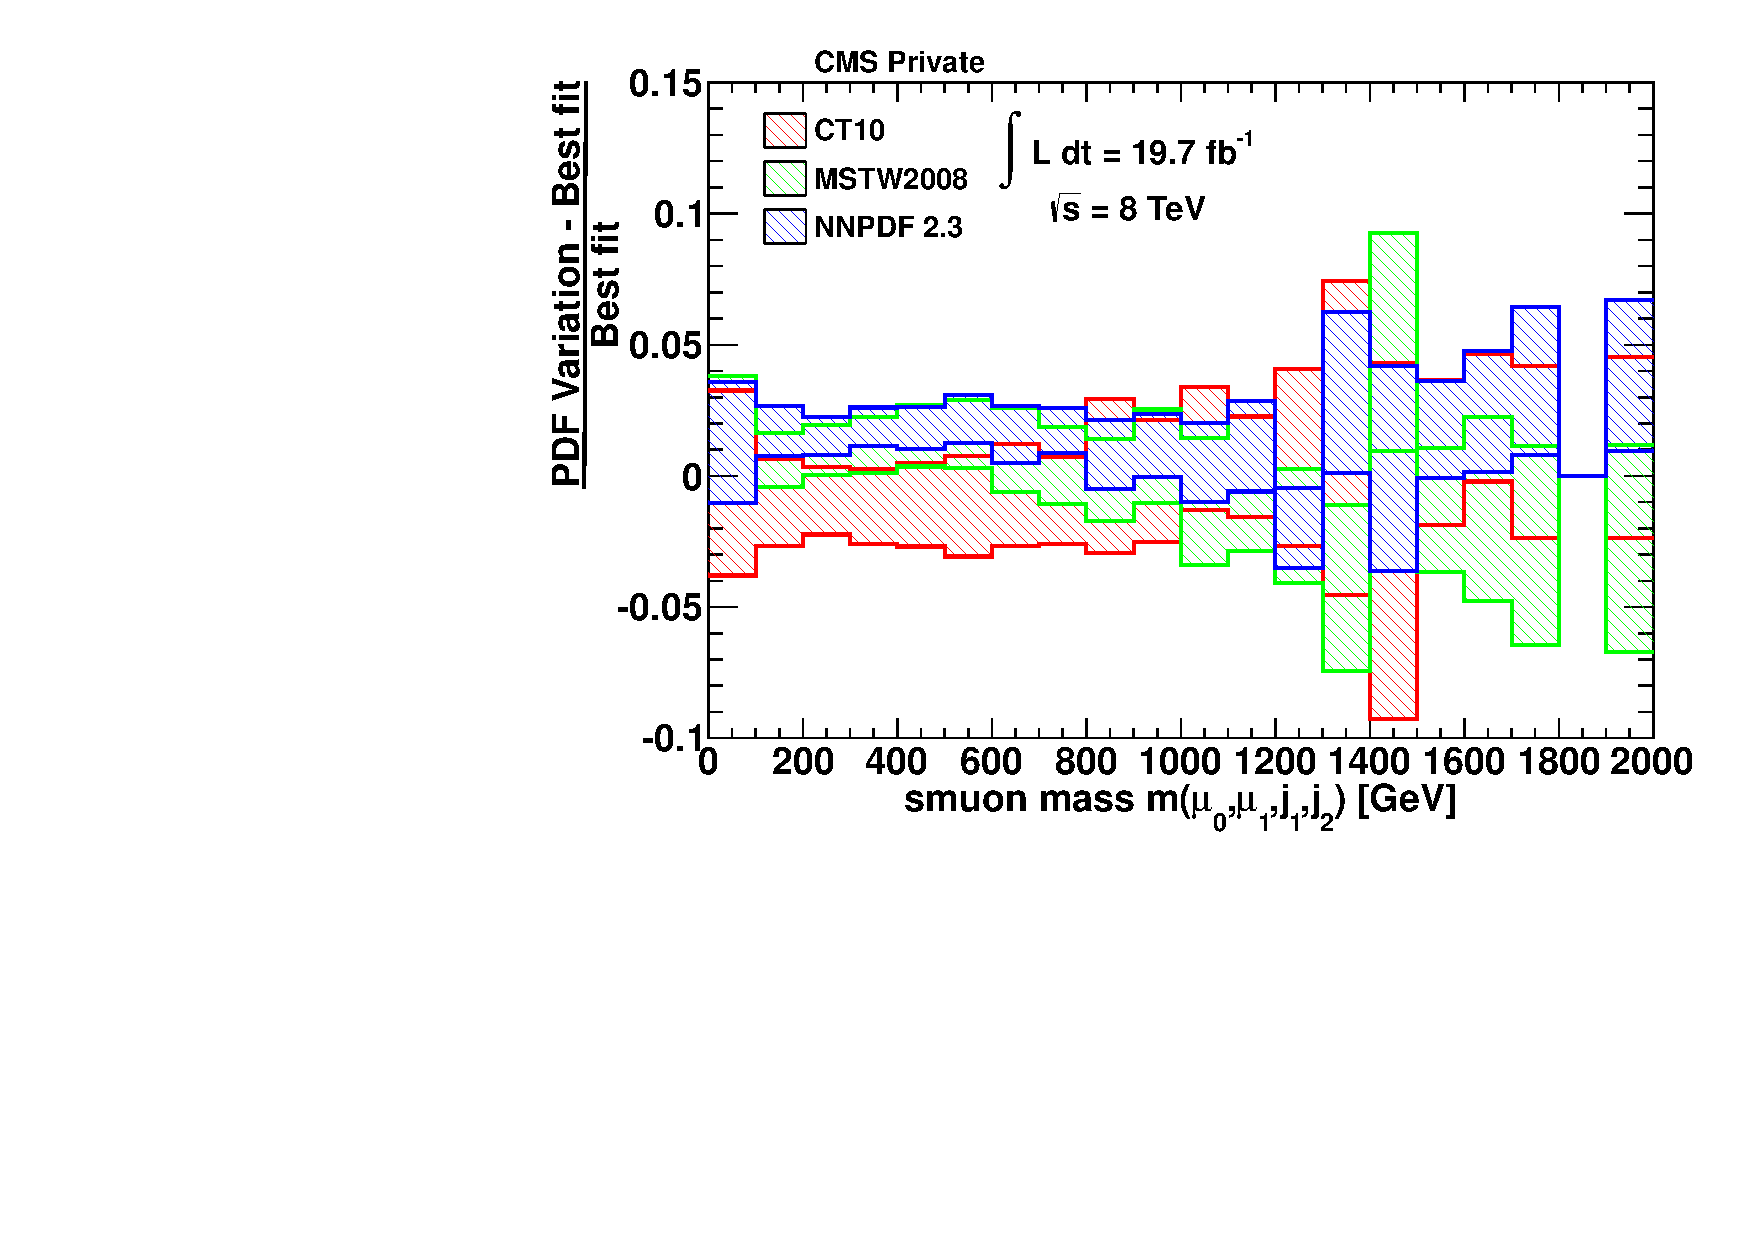
\includegraphics[width=0.7\textwidth]{plots/pdfratios.pdf}
  \caption{PDF uncertainties for all background Monte Carlo samples for the smuon mass. They are given relative to the best fit calculated from the three PDF sets.}
  \label{fig:pdfsys}
\end{figure}

Towards higher masses ($\geq 1000\,\text{GeV}$) the distribution lacks the necessary number of entries to yield statistically significant results. Taking this into account, the overall systematic uncertainty introduced by PDFs is estimated to be a flat $\pm 6\,\pct$.

For the signal Monte Carlo, the authors of the cross section calculation tool estimate a $5\,\pct$ uncertainty~\cite{susyxstool}, which is being used in this analysis.


\subsection{Pileup}
\label{sec:pusys}

For the pileup reweighting procedure, there are mainly two systematic uncertainties that contribute to determining the number of interactions~\cite{pileupsys}. The measurement of the bunch luminosity and the total inelastic cross section. The latter has been determined through the comparing the number of vertices in $Z \rightarrow \mu\mu$ events between simulation and measurement. A $3.9\,\pct$ uncertainty is attributed to this procedure. The $2.6\,\pct$ error on the luminosity has already been discussed in section~\ref{sec:lumisys}.

Additional uncertainties arise from possible shifts in the reweighting and pileup modelling processes, as well as potential beam size variations over time. They are expected to be small, but are taken into account by shifting the number of interactions by an overall amount of $\pm 5\,\pct$. The impact of this shift amounts to $-1.1\,\pct$ and $+1.5\pct$. For the signal Monte Carlos, the effect lies between $0.3\,\pct$ and $0.8\,\pct$.


\subsection{Trigger Efficiency}
\label{sec:trig-eff}

The performance of the trigger may vary between data and simulation. To account for this, trigger efficiency scale factors, which are the ratio between the efficiencies in Monte Carlo and data, are determined. Figure~\ref{fig:triggereff} shows a comparison of the ``turn on'' curves in 2012 jet data and the $t\bar{t}$ Monte Carlo.

\begin{figure}[!htb]
  \centering
  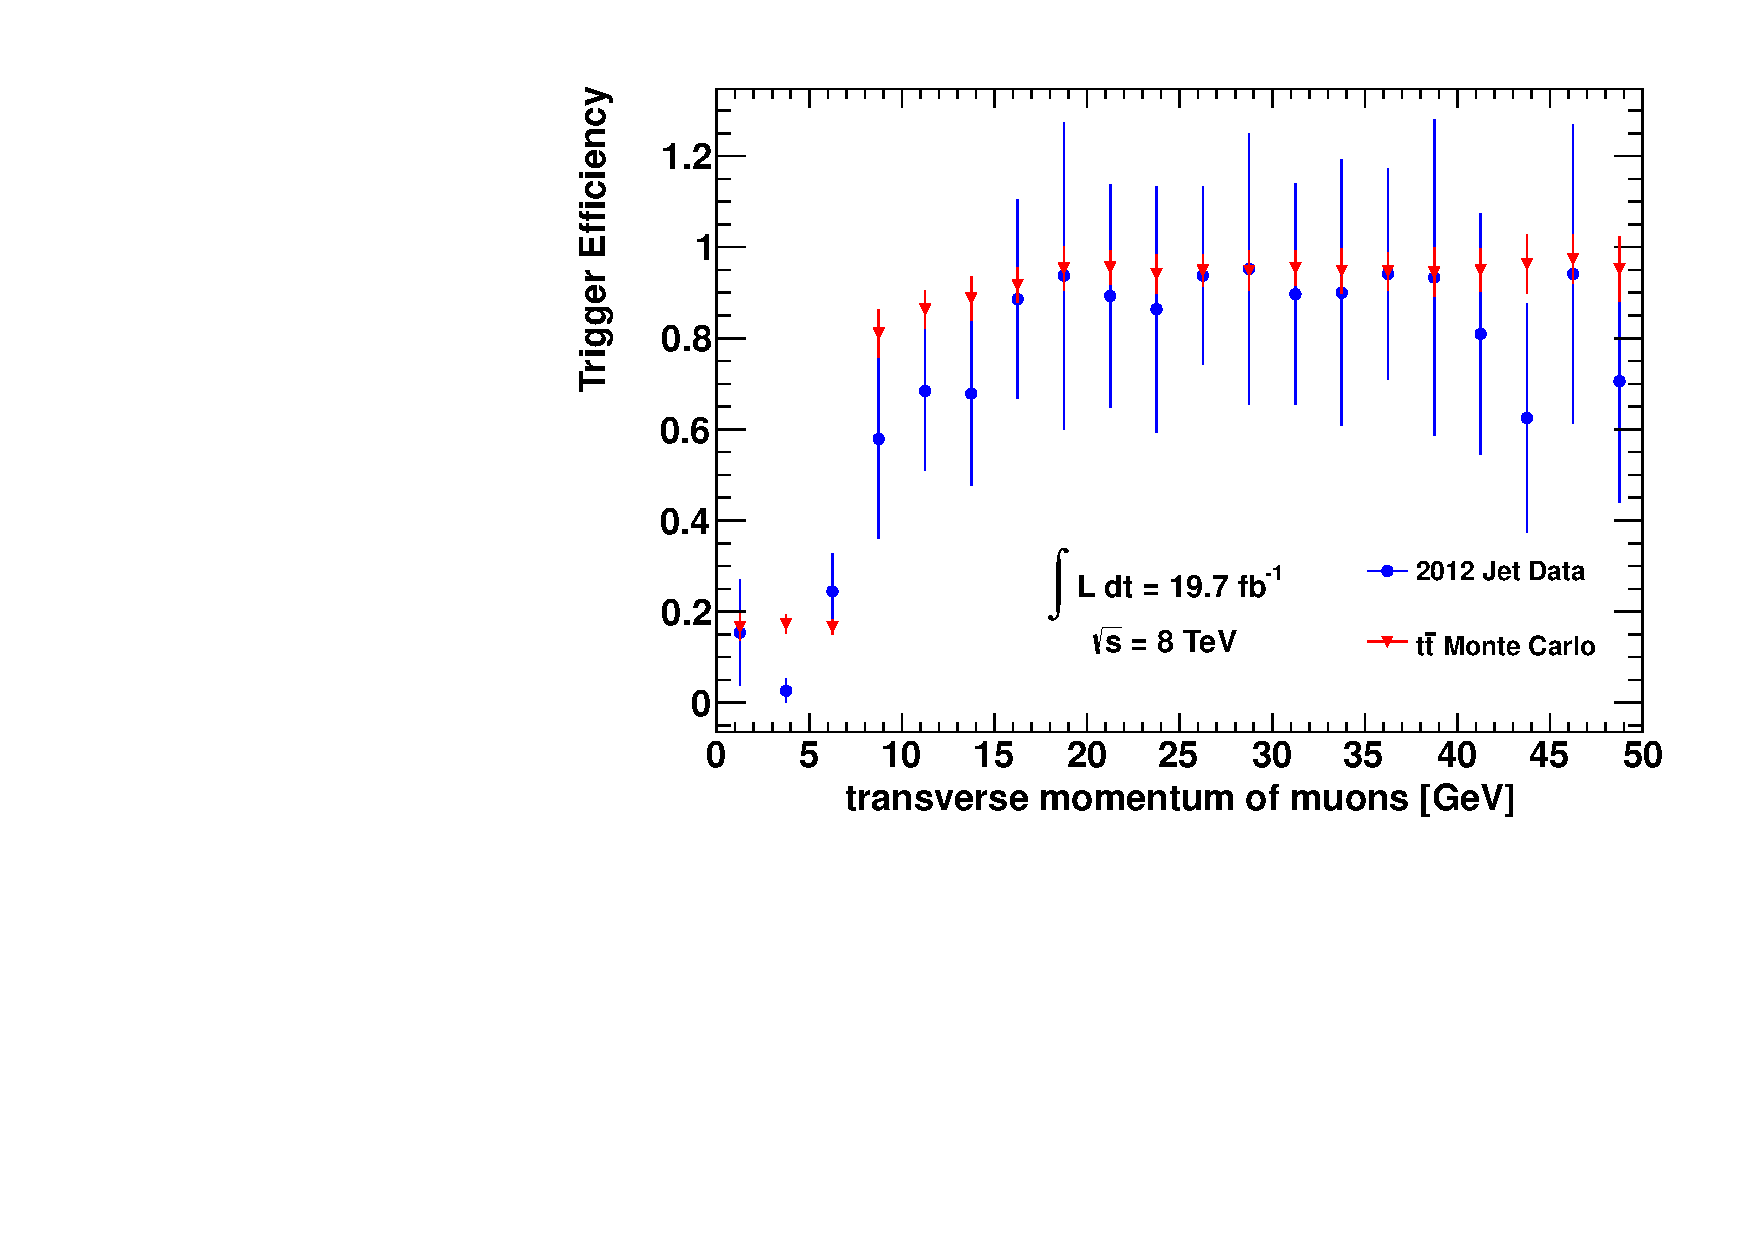
\includegraphics[width=0.7\textwidth]{plots/trigger_eff.pdf}
  \caption{Trigger efficiencies for 2012 jet data and $t\bar{t}$ Monte Carlo~\cite{teyssier}. The resulting scale factor is used to account for the discrepancy.}
  \label{fig:triggereff}
\end{figure}

Both distributions are created right before the application of the same sign charge requirement. By including the latter, one would reduce the already low statistics to a point where the result is dominated by its statistical errors. Due to the nature of this analysis, implementing scale factors for muons depending on their transverse momentum can lead to moderately complex individual event weights. To avoid this issue, keeping the transverse momentum threshold of $15\,\text{GeV}$ for the sub-leading muon in mind, a conservative $5\,\pct$ systematic uncertainty is assumed as compensation.

\section{Fake Rate Uncertainties}
\label{sec:tlsys}

Determining the tight-to-loose ratio $F_R$ varies depending on the chosen requirements for the QCD multi-jet enrichment of the sample. To estimate the systematic uncertainty introduced by this method, a single quantity is varied, while the others are kept constant. As opposed to the previously discussed systematic uncertainties, the impact on the number of events can be within the expected statistical variation. Should this be the case, it cannot be considered a systematic uncertainty. Calculating the variation is based on how the relative systematic uncertainty $\sigma_{\text{sys}}$ is determined. With the number of events from the default method as a reference $N_{\text{def}}$ and the one from the variation denoted by $N_{\text{var}}$, it is given by

\begin{equation}
  \label{eq:frsysabs}
  \sigma_{\text{sys}} = \frac{N_{\text{var}} - N_{\text{def}}}{N_{\text{def}}}.
\end{equation}

\noindent The statistical uncertainty then follows as

\begin{equation}
  \label{eq:frstatabs}
  \sigma_{\text{stat}} = \frac{\sqrt{\sigma_{\text{var}}^2 - \sigma_{\text{def}}^2}}{N_{\text{def}}}.
\end{equation}

\noindent Note that one would usually expect the $\sigma$ to be \textit{added} in quadrature. However, this uncertainty would correspond to the number of events instead of the method itself. Since these values are strongly correlated, they are required to be subtracted.

Table~\ref{tab:tlratiosys} shows the results of the variations.

\begin{table}[htb!]
  \centering
  \begin{tabular}{|l|c|c|}
    % BEGIN RECEIVE ORGTBL tlratiosys
\hline
Quantity & Variation & Impact on estimate $[\pct]$ \\
\hline
\hline
Comb. Rel. Iso. & 0.2 & $3.7 \pm 21.7$ \\
(default $< 0.5\,\text{GeV}$) & 0.4 & $1.7 \pm 4.6$ \\
 & 0.8 & $4.0 \pm 4.9$ \\
 & 1.0 & $5.1 \pm 5.4$ \\
\hline
$p_{\text{T, jet}}$ & 40 & $7.6 \pm 3.9$ \\
(default $> 50\,\text{GeV}$) & 60 & $-5.8 \pm 3.1$ \\
 & 70 & $-9.3 \pm 3.6$ \\
\hline
$E_{\text{T}}^{\text{miss}}$ & 40 & $0.6 \pm 0.5$ \\
(default $< 50\,\text{GeV}$) & 60 & $-0.9 \pm 1.4$ \\
 & 70 & $-2.1 \pm 2.1$ \\
\hline
$m_{\text{T}}(\mu, E_{\text{T}}^{\text{miss}})$ & 30 & $-3.8 \pm 2.4$ \\
(default $< 40\,\text{GeV}$) & 50 & $8.6 \pm 4.3$ \\
 & 60 & $14.2 \pm 5.9$ \\
\hline
    % END RECEIVE ORGTBL tlratiosys
  \end{tabular}
  \caption{Parameter variations to determine the systematic uncertainties of determining the fake rate $F_R$. Only one requirement is varied at a time. The expected statistical deviation has to be kept in mind.}
  \label{tab:tlratiosys}
\end{table}

\begin{comment}
#+ORGTBL: SEND tlratiosys orgtbl-to-latex :splice t :no-escape t
|-------------------------------------------------+-----------+-----------------------------|
| Quantity                                        | Variation | Impact on estimate $[\pct]$ |
|-------------------------------------------------+-----------+-----------------------------|
|-------------------------------------------------+-----------+-----------------------------|
| Comb. Rel. Iso.                                 |       0.2 | $3.7 \pm 21.7$              |
| (default $< 0.5\,\text{GeV}$)                   |       0.4 | $1.7 \pm 4.6$               |
|                                                 |       0.8 | $4.0 \pm 4.9$               |
|                                                 |       1.0 | $5.1 \pm 5.4$               |
|-------------------------------------------------+-----------+-----------------------------|
| $p_{\text{T, jet}}$                             |        40 | $7.6 \pm 3.9$               |
| (default $> 50\,\text{GeV}$)                    |        60 | $-5.8 \pm 3.1$              |
|                                                 |        70 | $-9.3 \pm 3.6$              |
|-------------------------------------------------+-----------+-----------------------------|
| $E_{\text{T}}^{\text{miss}}$                    |        40 | $0.6 \pm 0.5$               |
| (default $< 50\,\text{GeV}$)                    |        60 | $-0.9 \pm 1.4$              |
|                                                 |        70 | $-2.1 \pm 2.1$              |
|-------------------------------------------------+-----------+-----------------------------|
| $m_{\text{T}}(\mu, E_{\text{T}}^{\text{miss}})$ |        30 | $-3.8 \pm 2.4$              |
| (default $< 40\,\text{GeV}$)                    |        50 | $8.6 \pm 4.3$               |
|                                                 |        60 | $14.2 \pm 5.9$              |
|-------------------------------------------------+-----------+-----------------------------|
\end{comment}
 
Only the listed quantities are examined. All of the other ones are motivated by trigger thresholds or analysis requirements. For example the transverse momenta thresholds for muons are restricted by the choice of the trigger and the dimuon mass window is limited by low mass resonances and the $Z$-peak. For the overall impact, the variations of the transverse momentum of jets and the transverse mass hypothesis are considered. For a given quantity, the average is taken and added in quadrature to the overall sum. With the combined relative isolation and missing transverse energy only yielding impacts which are within the expected variation, they do not contribute.


\subsection{Closure Test}
\label{sec:closure-test}

To quantify the difference between the tight-to-loose ratio $F_R$ of the recorded data and the Monte Carlo prediction of the ratio given by the QCD multi-jet background (Fig.~\ref{fig:tlratios}), a ``closure test'' is used. It provides a test of concept for the data-driven background method, as well as being an indicator for the accuracy of the MC prediction. The general idea is to apply the tight-to-loose ratio $F_R$ to a chosen background and compare the result to its Monte Carlo prediction. A comparison between the tight-to-loose ratios measured in data and the QCD multi-jet counterpart it is meant to be similar to, yields the aforementioned quality estimate for the method itself. Since the $t\bar{t}$ background is the most prominent one in the final stage of the analysis, it is used as the benchmark process in this test. Figure~\ref{fig:closuretest} shows both the proof of concept on the left, as well as the actual comparison on the right.

\begin{figure}
  \centering
  \begin{subfigure}[b]{0.495\textwidth}
    \centering
    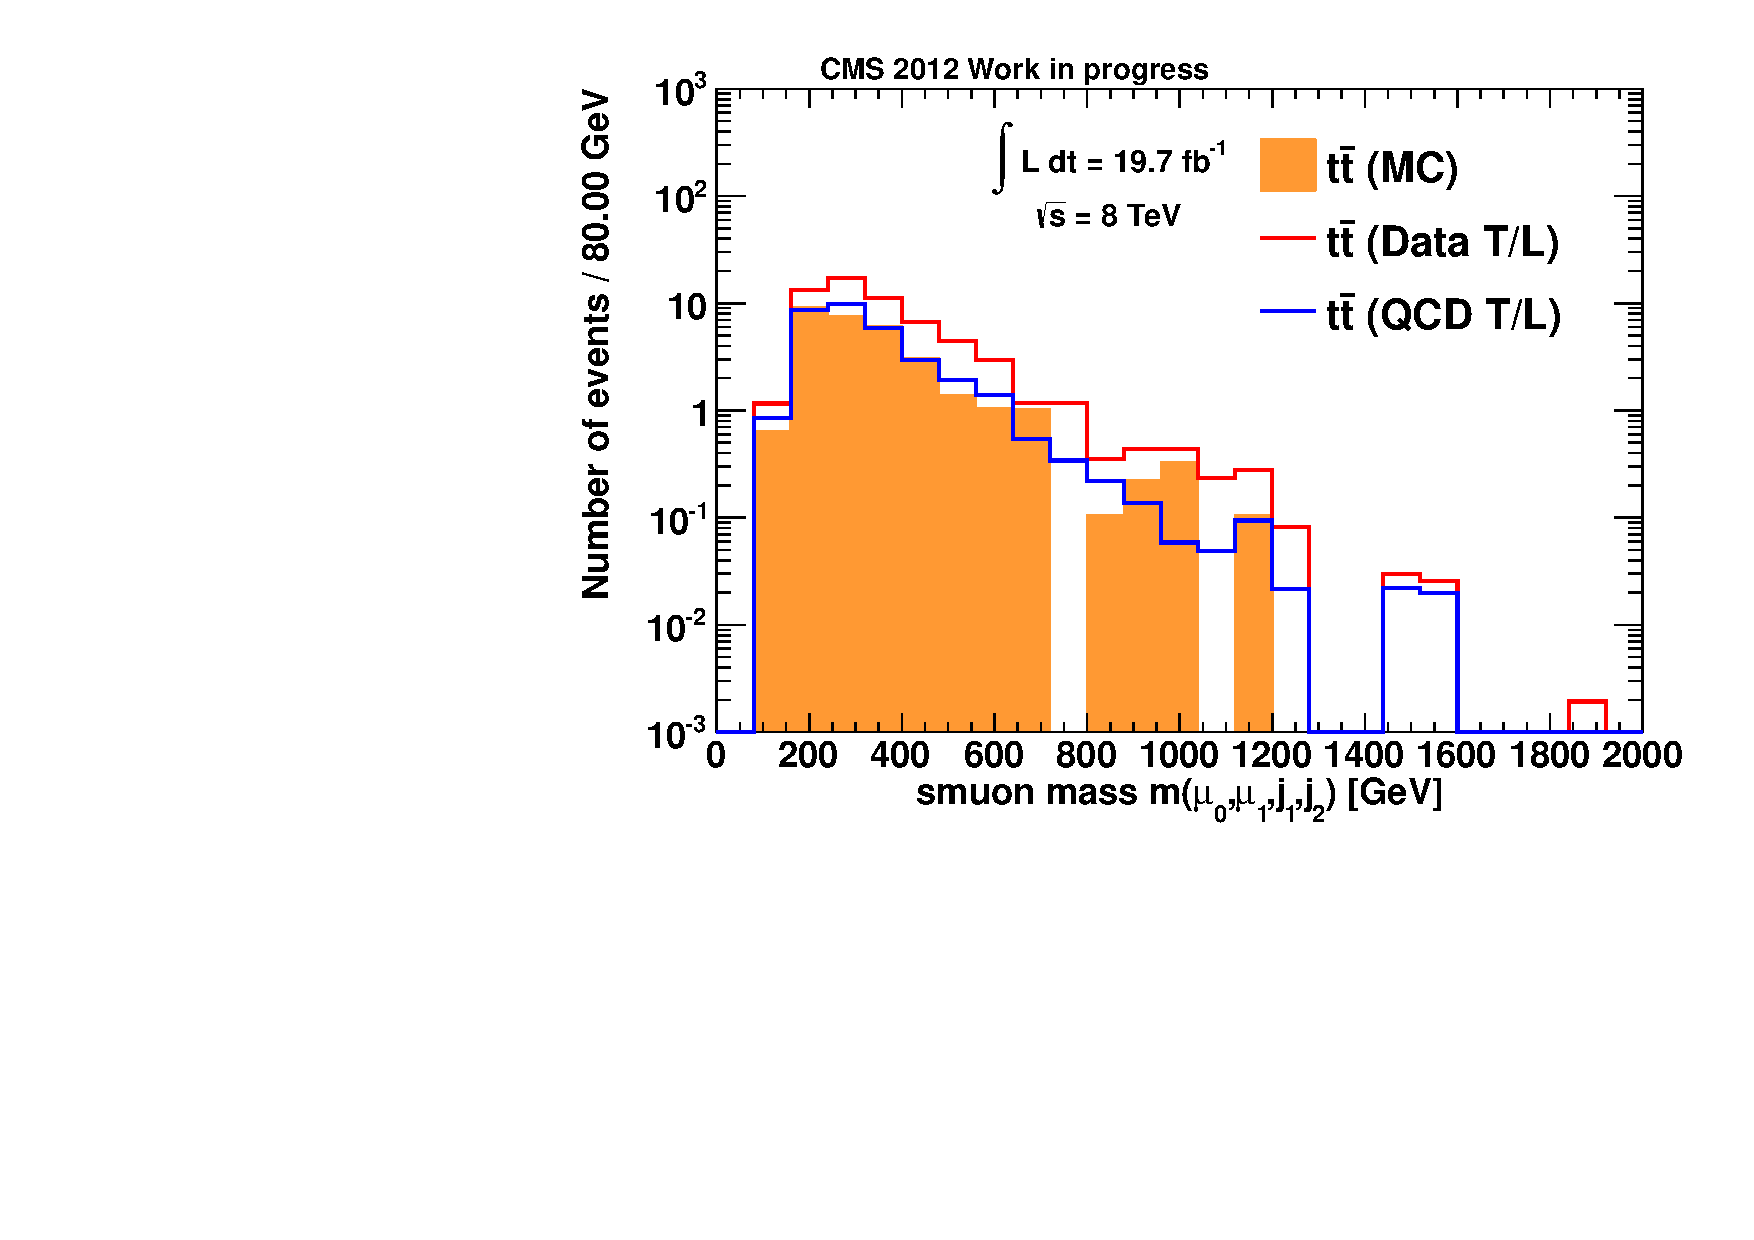
\includegraphics[width=\textwidth]{plots/closure_proof.pdf}
    \caption{\label{fig:closureproof}}
  \end{subfigure}
  \begin{subfigure}[b]{0.495\textwidth}
    \centering
    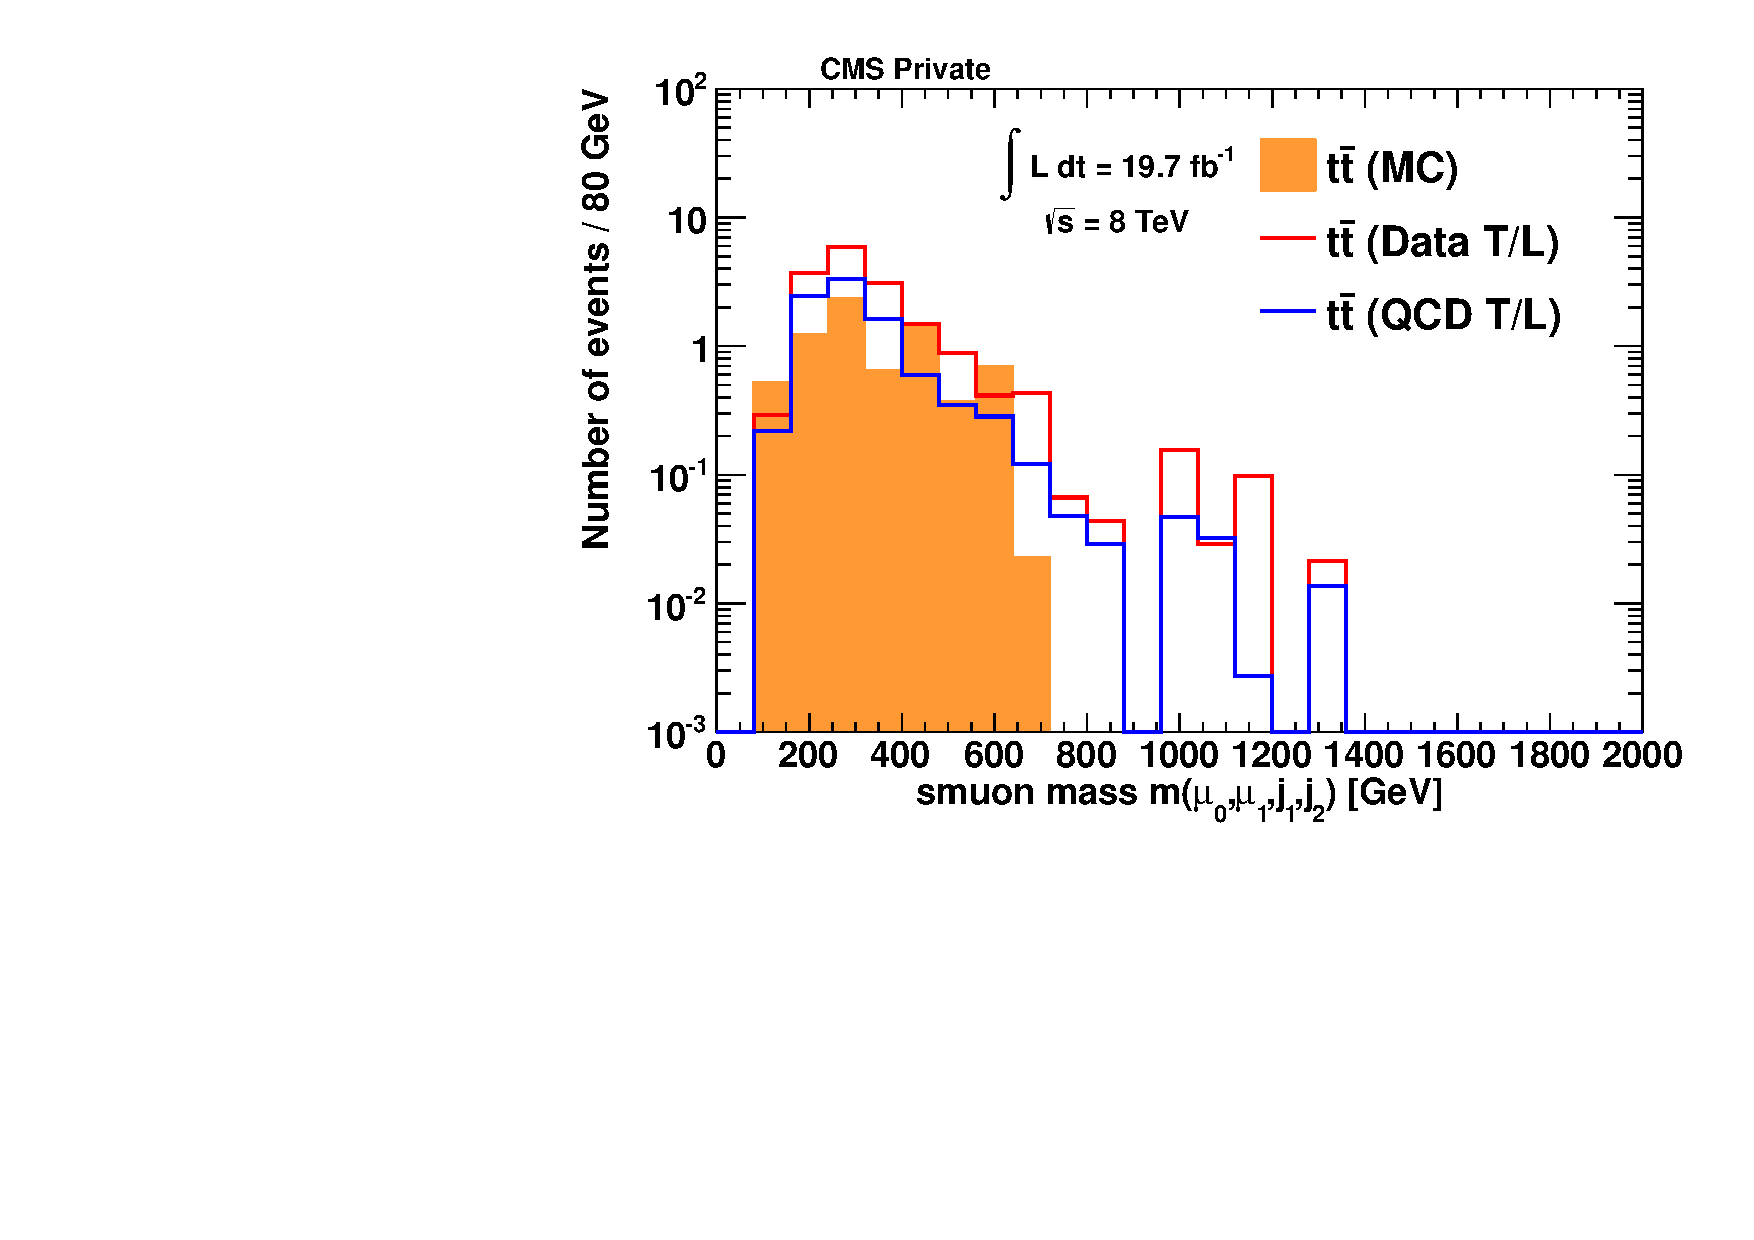
\includegraphics[width=\textwidth]{plots/closure_test.pdf}
    \caption{\label{fig:closurecomparison}}
  \end{subfigure}

  \caption{Proof of concept provided by the closure test (\ref{fig:closureproof}) and comparison between QCD multi-jet and data tight-to-loose ratios $F_R$ in the smuon mass distribution (\ref{fig:closurecomparison}). Both distributions show the Monte Carlo prediction, as well as both the QCD multi-jet and the data tight-to-loose ratio applied to it. While the right distribution was filled at the final stage, the left one is filled at the charge control region.}
  \label{fig:closuretest}
\end{figure}

To provide a proof of concept for the fake rate method, the charge control region CRC is being used. Aside from the typical inverted $E_{\text{T}}^{\text{miss}}$ requirement, it is characterised by not applying the $b$-jet veto while requiring the same charge one. For the proof the QCD multi-jet tight-to-loose ratio is measured and applied to the $t\bar{t}$ background. It is shown alongside the corresponding $t\bar{t}$ Monte Carlo. Note that the ratio measured in data cannot be used here, as the previously observed difference to the Monte Carlo tight-to-loose ratio already implies a differing result. The good agreement between the QCD multi-jet $F_R$ and MC prediction that can be seen in figure~\ref{fig:closureproof}, is an indication for the quality of the method itself.

The actual comparison of the results of applying both the data and the QCD multi-jet tight-to-loose ratio to the $t\bar{t}$ background is shown in figure~\ref{fig:closurecomparison}. Since one initially expected comparable results from both predictions, their disagreement of $45\,\pct$ in the number of events is taken as a systematic uncertainty.

While all previously discussed uncertainties apply to the Monte Carlo samples that are used for the statistical subtraction, their overall impact is reduced significantly. As they affect \textit{both} the number of tight and loose muons, calculating the ratio absorbs a large portion of this impact. Since the relative contributions of the individual uncertainties to the tight and loose subsets are similar, they only play a comparatively minor role.

Taking the second order effects from the Monte Carlo subtraction and the luminosity uncertainty for the \textit{data}-driven estimate into account, a $47\,\pct$ systematic uncertainty is assumed for the fake rate method.


\section{Summary}
\label{sec:summary}

In table~\ref{tab:sys-uncertainties}, the systematic uncertainties on the overall number of events are summarized. From the individual impacts of the up- and downward variations, the larger value has been taken to remain conservative.

\begin{table}[!htb]
  \centering
  \begin{tabular}{|l|c|c|}
    % BEGIN RECEIVE ORGTBL sys-uncertainties
    \hline
    Source of sys. uncertainty      & Background Impact $[\pct]$ & Signal Impact $[\pct]$ \\
    \hline
    \hline
    Jet Energy Resolution           & 0.6                        & 2.6                    \\
    Jet Energy Scale                & 3.6                        & 7.8                    \\
    Muon Momentum Resolution        & 0.2                        & 1.0                    \\
    Muon Momentum Scale             & 0.2                        & 3.0                    \\
    Muon ID Efficiency              & 1.0                        & 1.0                    \\
    B-Tagging                       & 0.6                        & 1.4                    \\
    \hline
    Luminosity                      & 2.6                        & 2.6                    \\
    Parton Distribution Functions   & 6.0                        & 5.0                    \\
    Cross sections                  & 17.3                       & 8.6                    \\
    Pileup                          & 1.5                        & 0.8                    \\
    Trigger Efficiency              & 5.0                        & 5.0                    \\
    \hline
    $\sum$                          & 19.6                       & 14.6                   \\
    \hline
    \hline
    Data-driven Background Estimate & 47.0                       & N/A                    \\
    \hline
    % END RECEIVE ORGTBL sys-uncertainties
  \end{tabular}
  \caption{Summary of all systematic uncertainties. The cross section uncertainties are either listed in table~\ref{tab:mcsamples} or assumed to be 5 and 50 percent for a higher order and a LO calculation, respectively. Here, the average impact of the cross section uncertainties on the smuon distribution is given.}
  \label{tab:sys-uncertainties}
\end{table}

\begin{comment}
#+ORGTBL: SEND sys-uncertainties orgtbl-to-latex :splice t :no-escape t
|---------------------------------+----------------------------+------------------------|
| Source of sys. uncertainty      | Background Impact $[\pct]$ | Signal Impact $[\pct]$ |
|---------------------------------+----------------------------+------------------------|
|---------------------------------+----------------------------+------------------------|
| Jet Energy Resolution           |                        0.6 |                    2.6 |
| Jet Energy Scale                |                        3.6 |                    7.8 |
| Muon Momentum Resolution        |                        0.2 |                    1.0 |
| Muon Momentum Scale             |                        0.2 |                    3.0 |
| Muon ID Efficiency              |                        1.0 |                    1.0 |
| B-Tagging                       |                        0.6 |                    1.4 |
|---------------------------------+----------------------------+------------------------|
| Luminosity                      |                        2.6 |                    2.6 |
| Parton Distribution Functions   |                        6.0 |                    5.0 |
| Cross sections                  |                       17.3 |                    8.6 |
| Pileup                          |                        1.5 |                    0.8 |
| Trigger Efficiency              |                        5.0 |                    5.0 |
|---------------------------------+----------------------------+------------------------|
| $\sum$                          |                       19.6 |                   14.6 |
|---------------------------------+----------------------------+------------------------|
|---------------------------------+----------------------------+------------------------|
| Data-driven Background Estimate |                       47.0 |                    N/A |
|---------------------------------+----------------------------+------------------------|
\end{comment}




%%% Local Variables: 
%%% mode: latex
%%% TeX-master: "document"
%%% End: 
